\documentclass[11pt,letterpaper,final] {article}

%%%%%%%%%%%%%%%%%%%%%%%%%%%%%%
% Packages
%%%%%%%%%%%%%%%%%%%%%%%%%%%%%%

	\usepackage[margin=1in]{geometry}
	\usepackage{amsmath}
	\usepackage{amsfonts}
	\usepackage{fancyhdr}
	\usepackage{graphicx}
	% \usepackage{apacite}
	% \usepackage{tikz}
	% \usepackage{setspace}
	% \usepackage{multicol}
	% \usepackage[left]{lineno}

%%%%%%%%%%%%%%%%%%%%%%%%%%%%%%
% Page styling
%%%%%%%%%%%%%%%%%%%%%%%%%%%%%%
	
	%%%%%%%%%%%%%%%%%%%%
	% Headers and footers
	%%%%%%%%%%%%%%%%%%%%
	
	\pagestyle{fancy}
	\renewcommand{\headrulewidth}{0pt}
	\fancyhead{}
	\fancyfoot{}
	\rhead{Page \thepage}
	\lhead{Test \#12}
	
	%%%%%%%%%%%%%%%%%%%%
	% Graphics path
	%%%%%%%%%%%%%%%%%%%%
	
	\graphicspath{{./assets/}}
	
	%%%%%%%%%%%%%%%%%%%%
	% Frontmatter
	%%%%%%%%%%%%%%%%%%%%
	
	% \title{The Title}
	% \author{The Author}
	% \date{\today}
	
	

%%%%%%%%%%%%%%%%%%%%%%%%%%%%%%
% Custom definitions
%%%%%%%%%%%%%%%%%%%%%%%%%%%%%%
	% Easy scientific notation
	\newcommand{\e}[1]{\ensuremath{\times 10^{#1}}}
	
	% Textual subscripts
	\newcommand{\sub}[1]{\ensuremath{_{\text{#1}}}}
	
	% Textual superscripts
	\newcommand{\super}[1]{\ensuremath{^{\text{#1}}}}

\begin{document}

% \linenumbers
% \maketitle

\paragraph{Question 01.} Fragile X syndrome is caused by a trinucleotide repeat expansionof the X-linked \textit{FMR1} gene, wherein an excess of 200 repeats is typically sufficient to constitute fullblown clinical disorder. This trinucleotide repeat prevents the expression of the fragile X mental retardation proteion (FMRP) for which the gene encodes (O'Donnell \& Warren, 2002). This results in elongation of dendritic spines, important for excitatory synaptic transmission and synaptic plasticity (Rudeli et al., 1985).

Following the identification of this gene and the protein for which encodes, studies in mouse models examining hippocampal synaptic plasticity suggested a connection between metabotropic glutamate receptor (mGluR) and the FX phenotype (Huber et al., 2002). Specifically, long-term depression (LTD) in the hippocampus can be triggered by activation of either postsynaptic NMDA receptors or of postsynaptic Gp1 mGluRs, with each being mechanistically distinct. In mGluR-mediated LTD, a rapid translation of mRNA in postsynaptic dendrites is required, and, unlike NMDA LTD, mGluR-LTD is not easily reversible (Oliet et al., 1997).

Subsequent experiments led to the hypothesis that Gp1 mGluR activation additionally stimulates the synthesis of FMRP which then acts as an inhibitor of further synthesis and LTD. FMRP additionally is thought to repress translation of other specific mRNAs, with a missense mutation in its RNA-binding domain inhibiting this functioning and results in severe mental retardation (Feng et al., 1997).

These and other studies in \textit{Fmr1} knockout mice led to the mGluR theory of FX, wherein it was hypothesized that overactive Gp1 mGluR signaling actively contributed to the FX phenotype, driven by the inability to synthesize functional FMRP that would otherwise negatively regulate this pathway. Further, it predicted that the administration of mGluR antagonists could dampen the protein synthesis triggered by their activation and partially rescue or even reverse the FX phenotype (Bear, Huber, \& Warren, 2004).

Indeed, clinical trials were conducted on this basis by Novartis with the drug mavoglurant. Although it proceeded to a Phase II/III open-label trial, it has been since discontinued, citing negative results and failure to meet the primary endpoint of significant improvements to abnormal behaviors among adolescents and adults with fragile X syndrome compared to placebo treatment (ClinicalTrials.gov Identifier: NCT01433354). Roche has also recently completed a Phase II study with RO4917523, although no results have yet been disclosed (ClinicalTrials.gov Identifier: NCT01015430). At this point it is not apparent whether the failures of the Novartis trial were due to an inadequacy of the mFluR theory of Fragile X (certainly preclinical data support the theory) or an inadequate dosage or outcome measures (there exists some controversy over whether tolerance develops to the drug and the scales used to measure behavioral and cognitive improvement have been panned as having poor resolution).

\paragraph{Question 02.} Given the preliminary evidence suggesting that high-intensity exercise during pregnancy produces certain brain malformation and behavioral deficits, the scientific community should begin a program of research to systematically determine any causal effects of such an exercise regiment on the child's health. Importantly, any such program of study should be attuned to the six principles of teratology (agent-specificity; species-specificity; dosage-specificity; temporal sequencing; individual differences; and interaction effects) such that a causal relationship (or lack thereof) can be definitively established. Additionally, these principles may be references in responsibly communicating the potential risk to the general public while waiting for the results of further experimentation.

Foremost, research conducted should pay mind to both the agent and species specificity of these effects: is all high-intensity exercise equally detrimental to the child's health, or are some types of exercise acceptable while others severely damaging? Likewise, do these effects hold true across species? Will animal models of this effect faithfully recapitulate the phenotype observed in humans, or are retrospective and other observational human studies the only option to study this malformation? (As it has been observed in both humans and sheep, there is at least preliminary evidence for it affecting multiple species. However, the biomechanics of quadrupeds and bipeds do significantly differ: perhaps the resulting phenotype is the same, but the causal agent differs and a bipedal animal model (i.e., a non-human primate model) would be more appropriate for experimental manipulation.)

Additionally, as it applies to both experimentation and responsible communication to the public, are concerns of dose response. That is, in communicating the potential risk to the public, it will be important to emphasize that not all exercise is bad, but that it appears, based off of initial evidence, that only high intensity exercise produces these effects and that perhaps mild to moderate intensity workouts should be adopted by expectant mothers instead until more conclusive answers emerge. In experimentation, a dose-response curve should be derived, evidencing the progression of damage to the child as a function of both intensity and frequency of exercise by the mother during pregnancy.

This leads also into interaction effects and whether a lower intensity but higher frequency exercise regiment is equally as detrimental to the child as high intensity but lower frequency exercise. It appears that the body of literature has not given any indication to whether this effect is observed; however, that the most accurate health recommendations can be made, it is neither a factor that should be overlooked in and research program. Moreover, does gestational period significantly interact with either of these factors? I.e., is there a temporal aspect to the damage? Is high intensity exercise in the first trimester beneficial, yet highly detrimental in the third?

Ultimately, these and related concerns should be definitely answered that expecting mothers are able to remain fit throughout their pregnancy without risking damage to their child. However, until such point that these questions are adequately resolved, high intensity exercise during pregnancy should, at a minimum, be discouraged, and less intense alternatives proposed.

\paragraph{Question 03.} Utilizing stem cell populations for tissue engineering offers both promises and challenges. For instance, stem cells are able to subsequently differentiate into many lineages; however, expansion of these cell populations in culture has the tendency to reduce their subsequent differentiation potential. Additionally, monitoring these cells' ongoing potential to differentiate into multiple lineages represents a costly and time-consuming process. This cost is only increased by the active maintenance of a particular cytokine milieu to direct the differentiation of these populations. Further, only a subset of the stem cell population will ultimately acquire the desired lineage-specific characteristics and this represents overall a largely uncontrolled process. Moreover, significant testing is required to evaluate the cell population.

Conversely, the use of committed cells offers a relatively easier solution in terms of isolation and maintenance of cell populations. These, unlike stem cells, can be easily grown out in culture without the loss or alteration of lineage-specific characteristics. Further, these do not require the specific and intensive monitoring that stem cells do to ensure the integrity of the specific lineage, nor must they be grown in a particular and expensive cytokine environment. There additionally exist often substantial regulatory burdens with respect to the use of stem cells that are not levied against committed cell types, facilitating translation into clinical practice. Neither does there exist the risk of abnormal or unexpected differentiation or teratoma formation \textit{in vivo} as with stem cell populations.

\paragraph{Question 04.} In arrhythmia, reentry occurs as the result of a unidirectional block caused by refractory cardiac tissue. The electrical signal will, as it propagates throughout the cardiac tissue, if timed poorly, then excite the muscle previously in its refractory period. (See Figure \ref{fig:00}.) This may ultimately result in heterogeneity of action potentials across the heart, leading to non-uniform contraction across the span of the cardiac muscle.

\begin{figure}[htp]
  \centering
    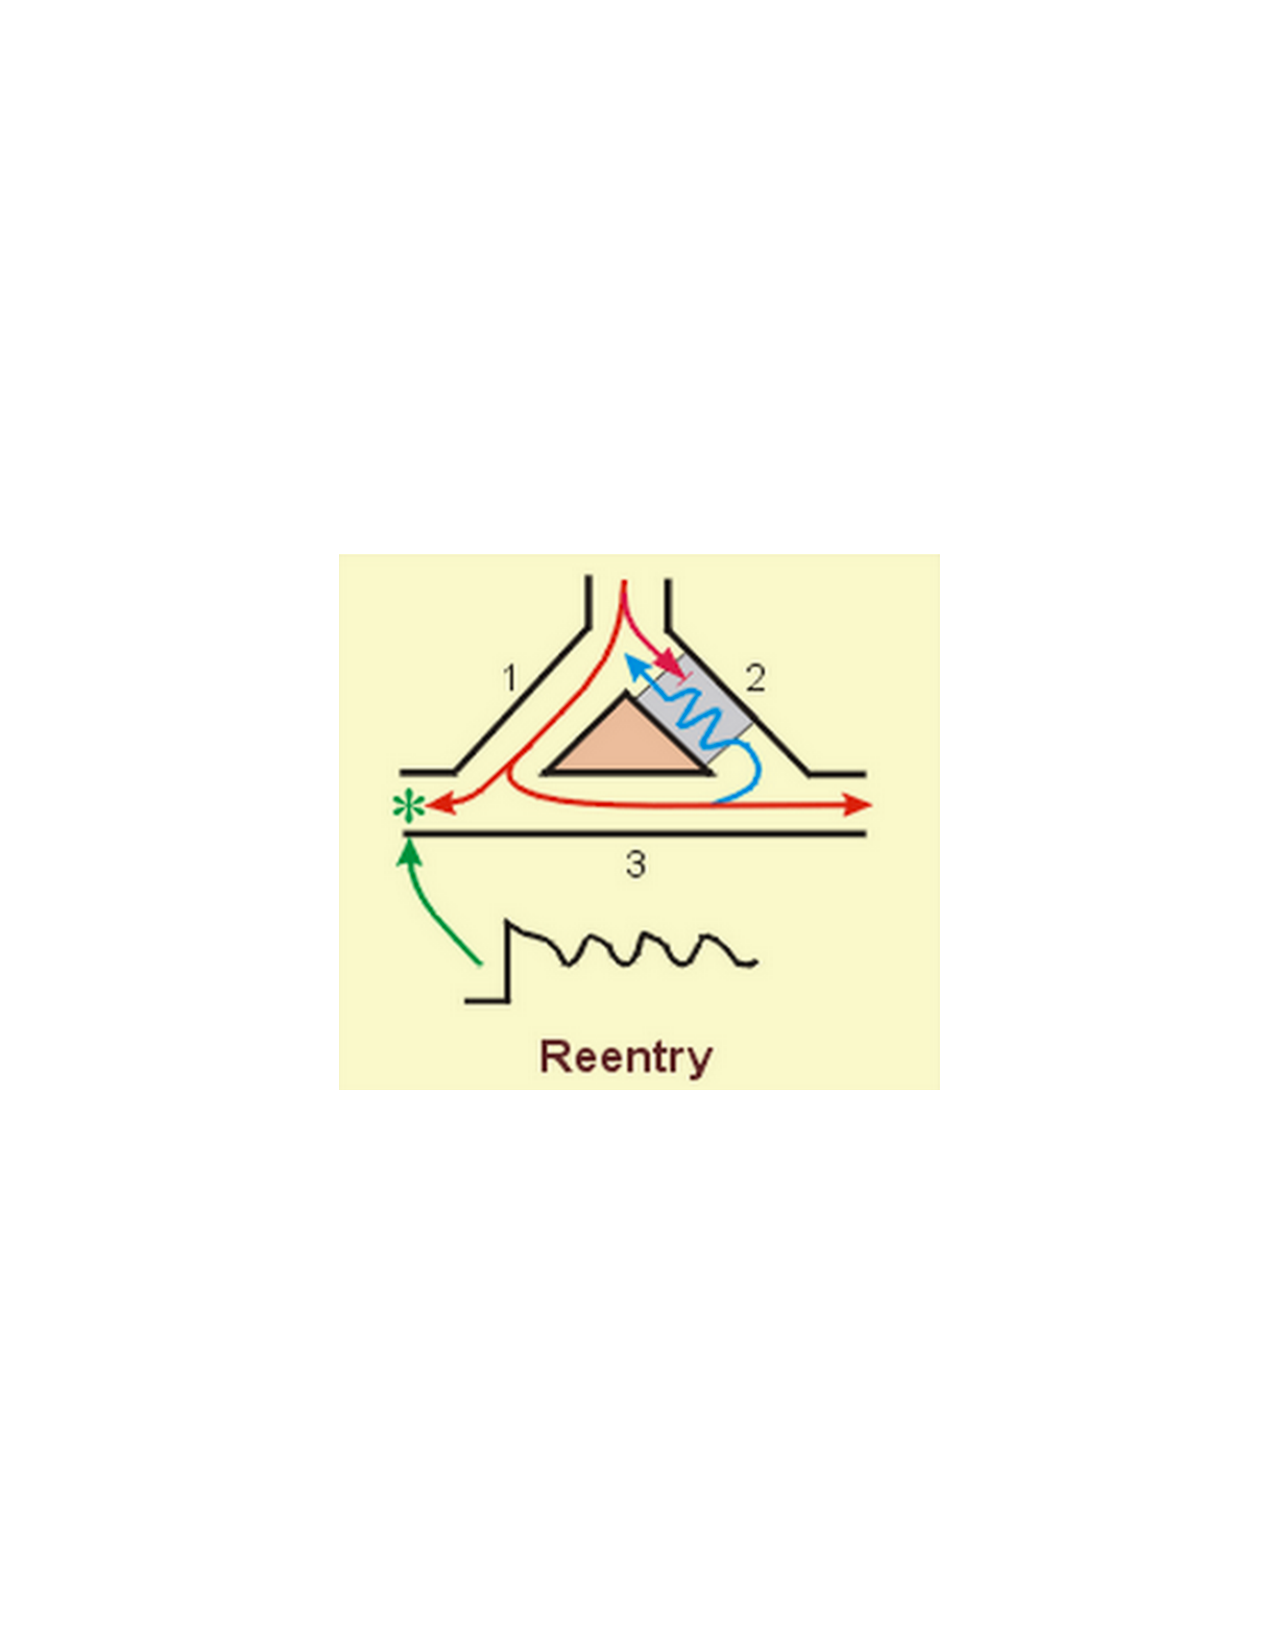
\includegraphics[width=0.45\textwidth]{reentry}
	\caption{Arrhythmia caused by reentry.}
	\label{fig:00}
\end{figure}

In the CAST trial, the investigators hypothesized that sodium channel blockers would reduce this occurrence as myocardiocytes are sodium channel gated. That is, by reducing cardiac cell excitability and slowing the flow of sodium ions into the cardiomyocyte,  the probability of hitting the calcium threshold potential will be decreased and, correspondingly, the cell will not depolarize as a function of stochastic ion movement, but only from legitimate action potentials.

However, these drugs unintentionally created a pro-arrhythmogenic environment from reentrant arrhythmias. Although, indeed, these drugs did reduce cellular excitability, they also created longer action potentials. In doing so, an action potential is then able to move through the ventricle and return to the originating cell, not while it is still in its refractory period, but when it is again able to be excited, resulting in a reentrant arrhythmia. Accordingly, this dramatically increased the risk of sudden cardiac death from an inability of the heart to any longer pump blood in a coordinated matter, having effectively decoupled the ventricle from the AV node.

\paragraph{Question 05.} Asthma begins development in childhood, often as a function of a genetically-determined sensitization risk attributable to delayed postnatal T\sub{H} cell maturation; developmental defects in T\sub{reg} cells; and an altered innate immune system (Anderson \& Cookson, 1999). Likewise, genome-wide association studies have identified evidence for asthma-related loci at genes for ``CHI3L1, IL6R, and DENND1B on chromosome 1, IL1RL1–IL18R1 on chromosome 2, PDE4D and RAD50–IL13 on chromosome 5, HLA-DQ on chromosome 6, IL33 on chromosome 9, SMAD3 on chromosome 15, ORMDL3-GSDMB on
chromosome 17, [and] IL2RB on chromosome 22'' (Martinez \& Vercelli, 2013).

In the sensitization to a new environmental protein, the incoming allergen will initially trigger pattern recognition receptors expressed by lung epithelial cells. These PRRs will then initiate the release of cytokines (primarily interleukin 1a), causing the release of additional pro-inflammatory cytokines, including granylocyte-macrophage colony-stimulating factor, IL-25, and IL-33 (Maddox \& Schwartz, 2002).

These expressed cytokines will then cause migration of dendritic cells, having sampled the antigen, to the draining lymph nodes, then presenting the allergen-derived peptide by an MHC-II molecule to a naive T cell. This cell will then differentiate into a T\sub{h}2 phenotype.

Upon re-exposure to the allergen, the T\sub{H}2 cells will be reactivated and induce production of IgE antibodies by B cells and additionally release pro-inflammatory cytokines such as IL-5, IL-9, and IL-13 that further induce eosinophilia, increase mast cell numbers in the lungs, and promote production of mucus by the lung epithelium. We further see remodeling of the airway, including thickening of the subepithelial tissue and narrowing of the airway lumen.

\paragraph{Question 06.} Among mice with the \textit{Myc} oncogene, translocation (t(8;14), t(8;22) or t(2;8)) is typically required for the onset of Burkitt lymphoma. Additionally, in leukemia and lung carcinoma, we may see its gene amplification. For tumorigenesis, however, we additionally must see downregulation of various checkpoint mechansims, including proliferative arrest, apoptosis, and cellular senescence (Gabay, Li, \& Felsher, 2014). Activation of \textit{Ras}, alternatively, induces inhibition of apoptosis through Bad, protein synthesis through mTOR, cell proliferation through GSK-3$\beta$, and cell cycle progression through FOXO. However, Ras alone is insufficient to immortalize cells, as demonstrated by Land et al. (1983). Recent work has demonstrated that c-myc has the potential to immortalize human primary prostate and breast epithelial cells, although this may be an uncommon event (Thibodeaux et al., 2009; Yaswen \& Stampfer, 2002). In any event, Myc \textit{alone} is regarded as insufficient to induce tumorigenesis and it is only in collaboration with other oncogenic events that this is observed (Murray et al. 1983; Compere et al. 1989; DeoCampo et al. 2000). Constitutive signaling of Ras, however, does allow unchecked cellular proliferation (Goodsell, 1999).

As such, activation of cellular Ras would appear to be necessary for tumorigenesis, even in animals already expressing Myc, whereas Myc activation in animals already expressing Ras only serves to amplify tumorigenesis, but is not necessary (Wang, Lisanti, \& Liao, 2011). Further, under expression of moth Ras and Myc, it seems likely that the rate of tumor production is so high as (1) constitutive Ras signaling is sufficient alone for tumorigenesis and (2) Myc in a non-linear fashion universally upregulates gene expression: that is, genes already upregulated in the absence of Myc are strongly upregulated in its presence, to a degree far greater than genes with low expression in its absence (Nie et al., 2012). As such, Myc likely serves to potentiate the effects of the already highly-expressed Ras, thus resulting in high levels of tumor production.

%%%%%%%%%%%%%%%%%%%%
%% REFERENCES
%%%%%%%%%%%%%%%%%%%%

% \clearpage
% \bibliographystyle{apacite}
% \bibliography{references}

\end{document}